%\hypertarget{___gatsby}{}
%\hypertarget{gatsby-focus-wrapper}{}
%\href{https://mukulrathi.com/}{}
%
%MUKUL RATHI
%
%\href{https://mukulrathi.com/about-me}{}
%
%About Me
%
%\href{https://mukulrathi.com/blog}{}
%
%Blog
%
%\hypertarget{creating-the-bolt-compiler-part-11}{%
%\subsection{Creating the Bolt Compiler: Part
%11}\label{creating-the-bolt-compiler-part-11}}

\hypertarget{top-of-page}{%
\chapter{Adding Inheritance and Method Overriding to Our
Language}\label{top-of-page}}

January 25, 2021

%\hypertarget{january-25-2021}{%
%\subsection{January 25, 2021}\label{january-25-2021}}
%
%\hypertarget{min-read}{%
%\subsection{7 min read}\label{min-read}}

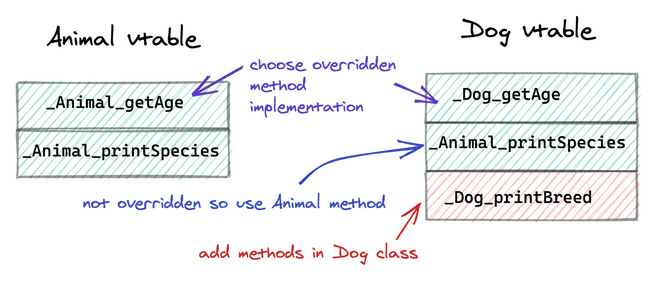
\includegraphics[width=\linewidth]{11_files/vtable.png}

%\hypertarget{series-creating-the-bolt-compiler}{%
%\section{Series: Creating the Bolt
%Compiler}\label{series-creating-the-bolt-compiler}}
%
%\begin{itemize}
%\item
%  { Part 1:
%  }\href{https://mukulrathi.com/create-your-own-programming-language/intro-to-compiler/}{How
%  I wrote my own "proper" programming language}
%\item
%  { Part 2:
%  }\href{https://mukulrathi.com/create-your-own-programming-language/compiler-engineering-structure/}{So
%  how do you structure a compiler project?}
%\item
%  { Part 3:
%  }\href{https://mukulrathi.com/create-your-own-programming-language/parsing-ocamllex-menhir/}{Writing
%  a Lexer and Parser using OCamllex and Menhir}
%\item
%  { Part 4:
%  }\href{https://mukulrathi.com/create-your-own-programming-language/intro-to-type-checking/}{An
%  accessible introduction to type theory and implementing a
%  type-checker}
%\item
%  { Part 5:
%  }\href{https://mukulrathi.com/create-your-own-programming-language/data-race-dataflow-analysis/}{A
%  tutorial on liveness and alias dataflow analysis}
%\item
%  { Part 6:
%  }\href{https://mukulrathi.com/create-your-own-programming-language/lower-language-constructs-to-llvm/}{Desugaring
%  - taking our high-level language and simplifying it!}
%\item
%  { Part 7:
%  }\href{https://mukulrathi.com/create-your-own-programming-language/protobuf-ocaml-cpp-tutorial/}{A
%  Protobuf tutorial for OCaml and C++}
%\item
%  { Part 8:
%  }\href{https://mukulrathi.com/create-your-own-programming-language/llvm-ir-cpp-api-tutorial/}{A
%  Complete Guide to LLVM for Programming Language Creators}
%\item
%  { Part 9:
%  }\href{https://mukulrathi.com/create-your-own-programming-language/concurrency-runtime-language-tutorial/}{Implementing
%  Concurrency and our Runtime Library}
%\item
%  { Part 10:
%  }\href{https://mukulrathi.com/create-your-own-programming-language/generics-parametric-polymorphism/}{Generics
%  - adding polymorphism to Bolt}
%\item
%  \textbf{Part 11: Adding Inheritance and Method Overriding to Our
%  Language}
%\end{itemize}
%
%\begin{center}\rule{0.5\linewidth}{0.5pt}\end{center}

Welcome back to part 11 of the series! We've got concurrency and
generics in our language, but we're still missing a key component:
\textbf{inheritance}. Remember, the four main OOP principles are

\begin{itemize}
\tightlist
\item
  Abstraction
\item
  Encapsulation
\item
  Inheritance
\item
  Polymorphism
\end{itemize}

Ah yes, there's polymorphism to tackle too. We've seen \emph{ad-hoc}
polymorphism, when we implemented
\href{https://mukulrathi.com/create-your-own-programming-language/lower-language-constructs-to-llvm/}{method
overloading in the desugaring stage}. We've seen \emph{parameteric}
polymorphism, when we implemented
\href{https://mukulrathi.com/create-your-own-programming-language/generics-parametric-polymorphism/}{generics}
last time round. In this post we'll cover the
\href{https://en.wikipedia.org/wiki/Polymorphism_(computer_science)}{third
type of polymorphism}: subtype polymorphism - \textbf{method
overriding}.

By the end of the tutorial, we'll be able to compile the following
program. We'll refer to this example to \emph{motivate} the changes
needed to the compiler, so that not only will you understand how the
changes work, but you'll understand \emph{why} they are implemented in
that way.

And hopefully, you'll be able to see the general principles we've used
to add generics in the last post, and inheritance and method overriding
in this post, so you'll be able to add even more language features going
forward!

%Copy

\begin{verbatim}
class Breed {...}
class Species { ... }
class Animal {  
   int age;  
   Species species;  
   int getAge() {    return this.age  }  
   void printSpecies(){ ... }
}

class Dog extends Animal {  
    Breed breed;  
    int getAge() {    return 7*this.age // dog years!  }  
    void printBreed(){ ... }
}

function void printAge(Animal a){  
   printf("I'm %d years old!", a.getAge());
}
void main() {  
  let animal = new Animal(age: 2);  
  let dog = new Dog(age: 2);
  printAge(animal) // print 2  
  printAge(dog) // print 14
}
\end{verbatim}

\hypertarget{just-give-me-the-code}{%
\section{\texorpdfstring{\protect\hyperlink{just-give-me-the-code}{}Just
give me the
code!}{Just give me the code!}}\label{just-give-me-the-code}}

As with the rest of the series, all the code can be found in the
\href{https://github.com/mukul-rathi/bolt}{Bolt repository}.

If you want to see the specific commits that were needed to implement
inheritance, check out
\href{https://github.com/mukul-rathi/bolt/pull/133}{this pull request}
and \href{https://github.com/mukul-rathi/bolt/pull/136}{this pull
request}.

\hypertarget{ast-definitions}{%
\section{\texorpdfstring{\protect\hyperlink{ast-definitions}{}AST
definitions}{AST definitions}}\label{ast-definitions}}

We need to store this inheritance relationship in our Abstract Syntax
Tree for our compiler to access. The easiest way is to store the name of
the superclass in the class definition, since we're reading it in when
we parse \texttt{CLASS\ Someclass\ EXTENDS\ Otherclass}:

%{
%\href{https://github.com/mukul-rathi/bolt/blob/master/src/frontend/parsing/parsed_ast.mli}{parsed\_ast.mli}}
%
%Copy

\begin{lstlisting}[language=caml,caption={parsed\_ast.mli}]
type class_defn = TClass of      Class_name.t      * generic_type option      * Class_name.t option (* optional superclass *)      * capability list      * field_defn list      * method_defn list
\end{lstlisting}

\hypertarget{type-checker}{%
\section{\texorpdfstring{\protect\hyperlink{type-checker}{}Type-Checker}{Type-Checker}}\label{type-checker}}

When we're adding a new language feature, we need to determine what
effect it has on the existing typing rules. With inheritance and method
overriding we have the following new rules:

\begin{itemize}
\tightlist
\item
  Subclasses like \texttt{Dog} have access to not only their own fields
  and methods, but also their superclass \texttt{Animal}'s fields and
  methods, (and the fields and methods of their superclass' superclass,
  and so on up the inheritance hierarchy).
\item
  Overridden methods (\texttt{getAge}) need to have the same type
  signature as their superclass (their return types need to match),
  since they're being used in the same contexts.
\item
  If a superclass is generic, then the subclass must also be generic -
  otherwise how could it access a field of generic type \texttt{T} in
  the superclass?
\item
  Subclasses like \texttt{Dog} are \textbf{subtypes} of their superclass
  (\texttt{Animal}). We have some new typing rules to handle when you
  can use \texttt{Dog} in place of \texttt{Animal}.
\end{itemize}

\hypertarget{accessing-superclass-methods}{%
\subsection{\texorpdfstring{\protect\hyperlink{accessing-superclass-methods}{}Accessing
superclass'
methods}{Accessing superclass' methods}}\label{accessing-superclass-methods}}

We just need to update the \texttt{get\_class\_methods},
\texttt{get\_class\_fields}, methods etc. to recursively look up the
method/field first in the current class, then its superclass and so on.

Here's a simple example: each class has a list of capabilities. With
inheritance, we do a recursive check to get the superclass' capabilities
too. The other \texttt{get\_class\_} methods are similar:

%{
%\href{https://github.com/mukul-rathi/bolt/blob/master/src/frontend/typing/type_env.ml\#L103-L125}{type\_env.ml}}
%
%Copy

\begin{lstlisting}[language=caml,caption={type\_env.ml}]
let rec get_class_capabilities class_name class_defns =  let open Result in  get_class_defn class_name class_defns Lexing.dummy_pos  >>= fun (Parsed_ast.TClass (_, _, maybe_superclass, capabilities, _, _)) ->  ( match maybe_superclass with  | Some superclass -> get_class_capabilities superclass class_defns  | None             -> Ok [] )  >>| fun superclass_caps -> List.concat [superclass_caps; capabilities]
\end{lstlisting}

\hypertarget{generics-and-inheritance}{%
\subsection{\texorpdfstring{\protect\hyperlink{generics-and-inheritance}{}Generics
and
Inheritance}{Generics and Inheritance}}\label{generics-and-inheritance}}

We pattern-match - if the current class isn't generic, and the
superclass is generic, raise a type error!

%{
%\href{https://github.com/mukul-rathi/bolt/blob/master/src/frontend/typing/type_env.type_inheritance\#L37-L47}{type\_inheritance.ml}}
%
%Copy

\begin{lstlisting}[language=caml,caption={type\_inheritance.ml}]
let type_generics_inheritance class_name curr_class_maybe_generic    (Parsed_ast.TClass (superclass_name, superclass_maybe_generic, _, _, _, _)) =  match (curr_class_maybe_generic, superclass_maybe_generic) with  | None, None | Some Generic, None | Some Generic, Some Generic -> Ok ()  | None, Some Generic ->      Error        (Error.of_string           (Fmt.str              "Type error: class %s must be generic since superclass %s is generic@."              (Class_name.to_string class_name)              (Class_name.to_string superclass_name)))
\end{lstlisting}

\hypertarget{method-overriding}{%
\subsection{\texorpdfstring{\protect\hyperlink{method-overriding}{}Method
overriding}{Method overriding}}\label{method-overriding}}

Remember, a method \emph{overrides} another if it has the same name and
parameter types (as \texttt{getAge} does in our example). To check the
overriding methods have the right type, we look up the method type
signatures of the current class and the superclass' methods. We raise an
error if the current class has a method that overrides an inherited
method (same method name and parameter types) but differs in return
type.

%{
%\href{https://github.com/mukul-rathi/bolt/blob/master/src/frontend/typing/type_env.type_inheritance\#L55-L79}{type\_inheritance.ml}}
%
%Copy

\begin{lstlisting}[caption={type\_inheritance.ml},language=caml]
let type_method_overriding class_name class_defns method_defns superclass_defn =  let open Result in  get_methods_type_sigs method_defns  |> fun methods_type_sigs ->  get_methods_type_sigs  (get_class_methods class_defns superclass_defn None Lexing.dummy_pos)  |> fun inherited_methods_type_sigs ->  List.filter    ~f:(fun (meth_name, ret_type, param_types) ->      List.exists        ~f:(fun (inherited_meth_name, inherited_ret_type, inherited_param_types) ->          meth_name = inherited_meth_name          && param_types = inherited_param_types          && not (ret_type = inherited_ret_type))        inherited_methods_type_sigs)    methods_type_sigs  |> function  (* we find any methods that violate overriding types *)  | []                     -> Ok ()  (* no violating methods *)  | (meth_name, _, _) :: _ ->      Error ...
\end{lstlisting}

\hypertarget{subtyping}{%
\subsection{\texorpdfstring{\protect\hyperlink{subtyping}{}Subtyping}{Subtyping}}\label{subtyping}}

We say a type \texttt{A} \emph{subtypes} type \texttt{B}, if we can use
\texttt{A} \textbf{in place of} \texttt{B}. That occurs if they're equal
(obvious) or if \texttt{A} is a subclass of \texttt{B} e.g. \texttt{Dog}
in place of \texttt{Animal}. Equivalently, we can say B is the
\emph{supertype} of A.

{
\href{https://github.com/mukul-rathi/bolt/blob/master/src/frontend/typing/type_env.type_inheritance\#L14-L20}{type\_inheritance.ml}}

Copy

\begin{lstlisting}[caption={type\_inheritance.ml},language=caml]
let is_subtype_of class_defns type_1 type_2 =  type_1 = type_2  ||  match (type_1, type_2) with  | TEClass (class_1, type_param_1), TEClass (class_2, type_param_2) ->      type_param_1 = type_param_2 && is_subclass_of class_defns class_1 class_2  | _ -> false
\end{lstlisting}

Intuitively the subtype, \texttt{A}, has \textbf{more info} than
\texttt{B}: the \texttt{Dog} class has all the \texttt{Animal} behaviour
and then some more behaviour specific to dogs.

When do we use subtyping?

\hypertarget{subtyping-in-variable-assignments}{%
\paragraph{\texorpdfstring{\protect\hyperlink{subtyping-in-variable-assignments}{}Subtyping
in Variable
Assignments}{Subtyping in Variable Assignments}}\label{subtyping-in-variable-assignments}}

We can assign subtypes to variables e.g.
\texttt{let\ x:\ Animal\ =\ new\ Dog()}. So in our \texttt{let}
expression typing judgement, we ensure the bound expr is a subtype of
the type annotation:

%{
%\href{https://github.com/mukul-rathi/bolt/blob/master/src/frontend/typing/type_expr.ml\#L88}{type\_inheritance.ml}}
%
%Copy


\begin{lstlisting}[caption={type\_inheritance.ml},language=caml]
| Parsed_ast.Let (loc, maybe_type_annot, var_name, bound_expr) ->      ...      type_with_defns bound_expr env      >>= fun (typed_bound_expr, bound_expr_type) ->        ( match maybe_type_annot with      | Some type_annot ->          if is_subtype_of class_defns bound_expr_type type_annot then Ok type_annot      ...
\end{lstlisting}

\hypertarget{subtyping-in-functions}{%
\paragraph{\texorpdfstring{\protect\hyperlink{subtyping-in-functions}{}Subtyping
in Functions}{Subtyping in Functions}}\label{subtyping-in-functions}}

Subtyping rules for functions are a little more complicated, so we'll
use our intuitive notion of subtypes having more info to help us out
here.

We can pass subtypes as arguments, as if the function \texttt{printAge}
was expecting an \texttt{Animal} and we give it a \texttt{Dog}, it can
ignore the extra info like \texttt{breed}. Here's the snippet of code
that does the check:

%{
%\href{https://github.com/mukul-rathi/bolt/blob/5543a135edc67bd8054141cbf99d68c44df59fb9/src/frontend/typing/type_overloading.ml\#L79-L80}{type\_overloading.ml}}
%
%Copy


\begin{lstlisting}[caption={type\_overloading.ml},language=caml]
...if are_subtypes_of class_defns args_types param_types then        Ok (param_types, return_type)...
\end{lstlisting}

Hold on, you ask, why is this subtype check in the
\texttt{type\_overloading} file?

Well, as you add language features, they start to interact with each
other.
\href{https://mukulrathi.com/create-your-own-programming-language/lower-language-constructs-to-llvm/}{Earlier
in the series}, we added function overloading: i.e. multiple functions
with the same name but different parameter types. We choose the correct
overloaded function based on the argument types: we pick the function
whose parameter types \emph{match}. Before, our definition of
\emph{match} was that the types were equal. Now, we say they
\emph{match} if the argument types are \textbf{subtypes} of the param
types.
\href{https://github.com/mukul-rathi/bolt/blob/master/src/frontend/typing/type_overloading.ml\#L89}{All
the details are in the code}.

Likewise, when type-checking our function return type, the body type
\emph{matches} the function return type, if it is a subtype. (If the
function returns \texttt{void} we don't care about the body type.)

%{
%\href{https://github.com/mukul-rathi/bolt/blob/master/src/frontend/typing/type_functions.ml\#L43}{type\_functions.ml}}
%
%Copy

\begin{lstlisting}[language=caml,caption={type\_functions.ml}]
...>>= fun (typed_body_expr, body_return_type) -> if return_type = TEVoid || is_subtype_of class_defns body_return_type return_type then    Ok ...else Error ...
\end{lstlisting}

An identical check is done to
\href{https://github.com/mukul-rathi/bolt/blob/master/src/frontend/typing/type_classes.ml\#L84}{type-check
methods}.

\hypertarget{lowering-to-llvm}{%
\section{\texorpdfstring{\protect\hyperlink{lowering-to-llvm}{}Lowering
to LLVM}{Lowering to LLVM}}\label{lowering-to-llvm}}

Now we've done the type-checking, we need to output LLVM IR in order to
run the program. Let's quickly remind ourselves of the program we're
trying to compile:

Copy

\begin{verbatim}
class Animal {  
  int age;  
  Species species;  
 int getAge() {    return this.age  } 
   void printSpecies(){ ... }
}

class Dog extends Animal {  
  Breed breed;  
  int getAge() {    return 7*this.age // dog years!  }  
  void printBreed(){ ... }
}

function void printAge(Animal a){  
   printf("I'm %d years old!", a.getAge());
}
void main() {
  let animal = new Animal(age: 2);
  let dog = new Dog(age: 2);
  printAge(animal) // print 2
  printAge(dog) // print 14
}
\end{verbatim}

\hypertarget{inheritance-and-structs}{%
\subsection{\texorpdfstring{\protect\hyperlink{inheritance-and-structs}{}Inheritance
and Structs}{Inheritance and Structs}}\label{inheritance-and-structs}}

Both the \texttt{Animal}and \texttt{Dog} classes are desugared to
structs containing their fields. This desugaring is straightforward for
\texttt{Animal}:

Copy

\begin{verbatim}
struct Animal {  int age;  Species *species;}
\end{verbatim}

Accessing the \texttt{age} field is desugared into getting a pointer to
field \texttt{0} of the struct, and likewise \texttt{species} is field
\texttt{1}.

On to the struct for \texttt{Dog}. We have three requirements:

\begin{itemize}
\tightlist
\item
  The struct needs to contain the fields in the \texttt{Dog} class.
\item
  It also needs to contain the fields in the \texttt{Animal} class.
\item
  A \texttt{Dog} struct should be able to be used wherever an
  \texttt{Animal} struct is expected.
\end{itemize}

The last point is the critical one. Say I have a \texttt{dog} object
being treated as an \texttt{Animal}. When I query \texttt{dog.age} and
\texttt{dog.species}, I'll expect them to be in field \texttt{0} and
\texttt{1} of the struct, since it's of type \texttt{Animal}. So the
\texttt{Dog} struct needs to preserve that field indexing. So the only
place the field \texttt{breed} can go is at index \texttt{2}.

Copy

\begin{verbatim}
struct Dog {  int age;  Species *species;  Breed *breed;}
\end{verbatim}

{
\href{https://mukulrathi.com/static/a759ba239e743d4372cd86fb6e9bc856/8affb/inheritance-struct.png}{{}
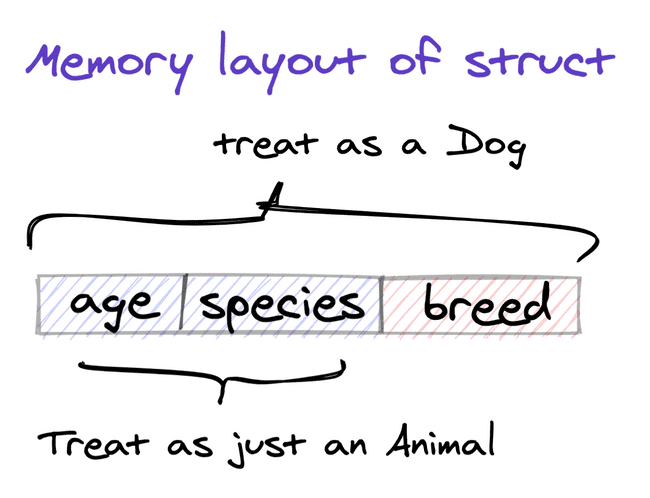
\includegraphics[width=\linewidth]{11_files/inheritance-struct.png}} }

In general, we order the struct so all the superclass's fields go first,
\emph{then} any fields declared in the current class. If we added a
subclass \texttt{Labrador}:

%Copy

\begin{verbatim}
class Labrador extends Dog{  Colour colour;}
// Desugared
struct Labrador {
  int age;
  Species *species;
  Breed *breed;
  Colour *colour;
}
\end{verbatim}

{
\href{https://mukulrathi.com/static/2ee5657d689e2e35a975960beace0cbb/a9577/another-inheritance-struct.png}{{}
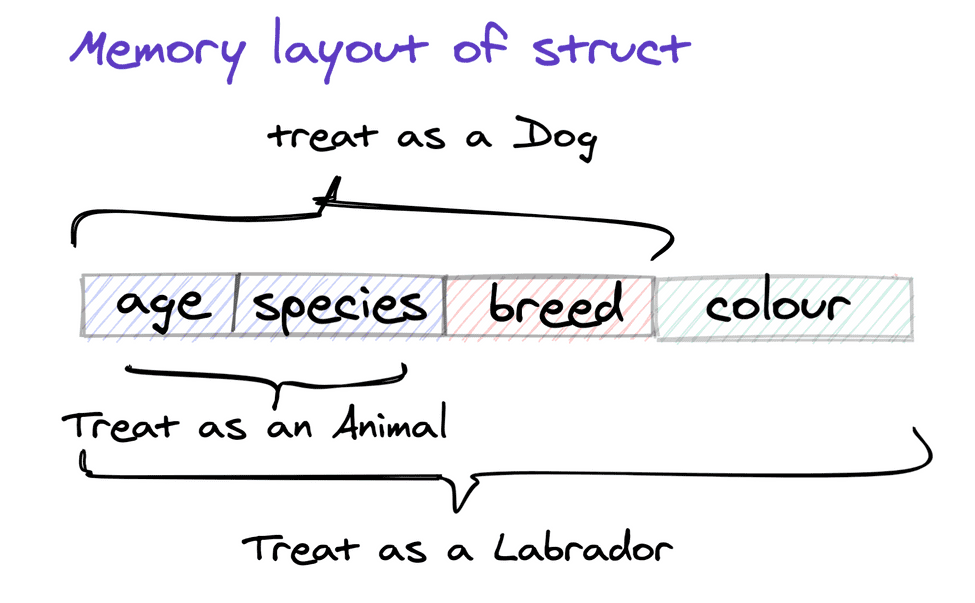
\includegraphics[width=\linewidth]{11_files/another-inheritance-struct.png}} }

If we want to treat a \texttt{Labrador} as an \texttt{Animal}, only look
at the first 2 fields. If you want to treat it as a \texttt{Dog} look at
the first 3 fields. And so on.

You can see this ordering in our \texttt{get\_class\_fields} method
during our IR generation stage, which puts \texttt{superclass\_fields}
first.

%{
%\href{https://github.com/mukul-rathi/bolt/blob/master/src/frontend/ir_gen/ir_gen_env.ml\#L17}{ir\_gen\_env.ml}}
%
%Copy

\begin{lstlisting}[language=caml,caption={ir\_gen\_env.ml}]
let rec get_class_fields class_name class_defns =  get_class_defn class_name class_defns  |> fun (TClass (_, maybe_superclass, _, fields, _)) ->  ( match maybe_superclass with  | Some super_class -> get_class_fields super_class class_defns  | None             -> [] )  |> fun superclass_fields -> List.concat [superclass_fields; fields]
\end{lstlisting}

Since we've handled this in the Bolt IR gen stage of the compiler
frontend, we don't need to change our LLVM backend, right?

Almost right. Just one hitch: LLVM IR is \textbf{typed}, so it will
complain if we pass a \texttt{Dog\ *} pointer to a function that expects
a \texttt{Animal\ *} pointer. Remember, LLVM has no notion of
inheritance, just raw structs, so it can't see that \texttt{Dog} is a
subclass of \texttt{Animal}. We thus \emph{explicitly cast} the argument
pointer to the function's expected param type before we pass it to the
function:

%{
%\href{https://github.com/mukul-rathi/bolt/blob/master/src/llvm-backend/llvm_ir_codegen/expr_codegen.cc\#L181-L191}{expr\_codegen.cc}}
%
%Copy

\begin{lstlisting}[language=C++,caption={expr\_codegen.cc}]
std::vector<Value *> argVals;  
for (int i = 0; i < expr.arguments.size(); i++) {
    Value *argVal = expr.arguments[i]->codegen(*this);
    Type *paramTy = calleeFunTy->getParamType(i);
    Value *bitCastArgVal = builder->CreateBitCast(argVal, paramTy);
    argVals.push_back(bitCastArgVal);  
}
\end{lstlisting}

\hypertarget{method-overriding-and-virtual-tables}{%
\subsection{\texorpdfstring{\protect\hyperlink{method-overriding-and-virtual-tables}{}Method
Overriding and Virtual
Tables}{Method Overriding and Virtual Tables}}\label{method-overriding-and-virtual-tables}}

Method overriding is a bit tricky, so take a breather.
\href{http://mukulrathi.co.uk/create-your-own-programming-language/lower-language-constructs-to-llvm/\#lowering-objects-to-structs}{From
our previous post}, we have that methods are desugared to regular
functions:

\begin{figure}
\centering
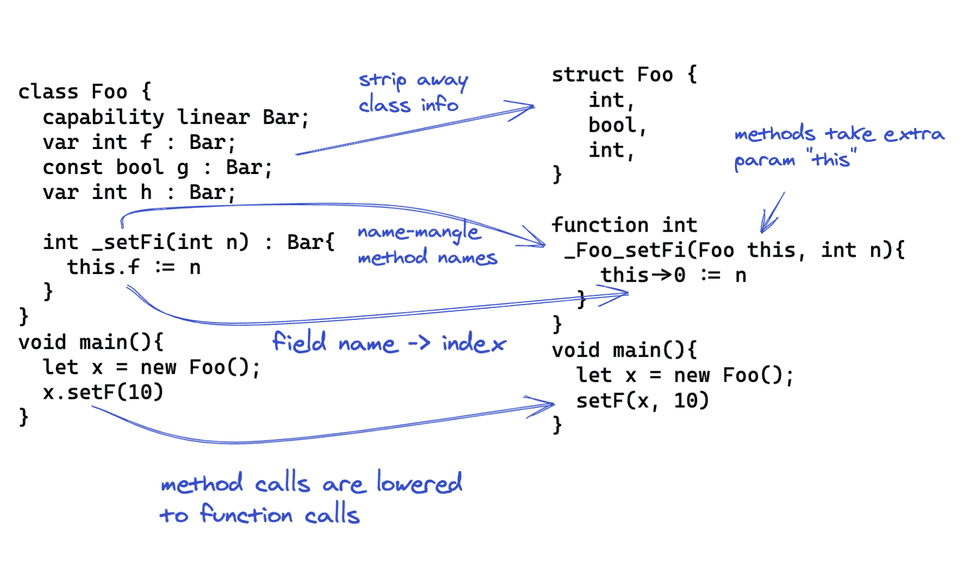
\includegraphics[width=\linewidth]{11_files/lower-classes.png}
\caption{The diagram from our previous desugaring post.}
\end{figure}

In our running example in this post we have \texttt{getAge} overridden,
so we have these two functions corresponding to the implementation of
\texttt{getAge} in each of the classes:

%Copy

\begin{verbatim}
Animal_getAge(Animal this){  return this.age}
Dog_getAge(Dog this){  return 7 * this.age}
\end{verbatim}

When we call \texttt{a.age()} in our \texttt{printAge} function, we want
to call \texttt{Animal\_getAge} if the underlying object is an
\texttt{Animal}, and \texttt{Dog\_getAge} if the object is actually a
\texttt{Dog}. The thing is, in general we don't know this information at
compile-time. Here's an example where type of \texttt{dog} is only known
at runtime:

%Copy

\begin{verbatim}
let dog = new Animal()
if (someCondition) {
  dog = new Dog()
}
dog.getAge() // which function do we call?
\end{verbatim}

So how do we insert the right call? The problem is not too dissimilar to
this:

%Copy

\begin{verbatim}
let dog = new Animal()
dog.age = 7
if (someCondition) {
  dog.age = 14
}
dog.age // which value does age have?
\end{verbatim}

We know how to do this: look up the value by indexing into the
\emph{list of fields} in the \texttt{dog} struct at runtime (index
\texttt{0} for \texttt{age}).

Since we've solved the problem for fields, let's do the same thing for
methods. We can create a \emph{list of (pointers to) methods} for each
class, called the \textbf{virtual table} or \textbf{vtable}. Instead of
determining the function call at compile-time, we instead provide an
\emph{index} into the table and call the function pointed to at that
index at runtime.

For similar reasons to the struct fields before, superclasses' methods
come before the current class's methods in the vtable. So we have
\texttt{getAge}, \texttt{printSpecies} first as they're from
\texttt{Animal}, then we have \texttt{getBreed} from \texttt{Dog}. To
override a method, we just replace its entry in the table:

{
\href{https://mukulrathi.com/static/c32dbd45d3466359a751c298568c0f5f/bfe41/vtable.png}{{}
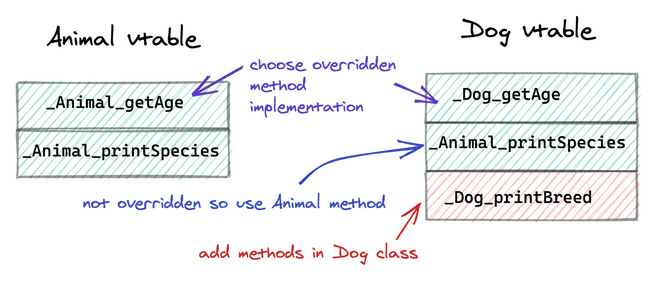
\includegraphics[width=\linewidth]{11_files/vtable.png}} }

Now we can just say for \texttt{dog.getAge()}, look at index \texttt{0}
of the \texttt{dog}'s vtable, and execute whichever function's there. Or
index \texttt{1} for \texttt{dog.printSpecies()}. \textbf{Problem
solved!}

\hypertarget{virtual-tables-in-our-structs}{%
\paragraph{\texorpdfstring{\protect\hyperlink{virtual-tables-in-our-structs}{}Virtual
Tables in our
structs}{Virtual Tables in our structs}}\label{virtual-tables-in-our-structs}}

Unlike fields, which are different for each object, vtables are the same
for \emph{all} objects of a \emph{given class}. Having a copy of the
same vtable in each object is wasteful: instead have just \textbf{one}
global vtable \textbf{per class}, and have the objects store a
\emph{pointer} to that.

We've reserved the first field in our object struct for the vtable
pointer:

%Copy

\begin{verbatim}
struct Animal {
  AnimalVTable *vtableptr;
  int age;
  Species *species;
}
struct Dog {
  DogVTable *vtableptr;
  int age;
  Species *species;
  Breed *breed;
}
\end{verbatim}

Okay, let's implement it with some code! To generate the vtable, we get
a list of the class' methods, \textbf{annotated} with the class they
came from (so we get the right overridden method). That is, we don't
have \texttt{getAge} we have the pair \texttt{(Dog,\ getAge)}. We use
this pair to generate the name-mangled function name:
\texttt{\_Dog\_getAge}. Our vtable is just a list of these name-mangled
function names.

%{
%\href{https://github.com/mukul-rathi/bolt/blob/master/src/frontend/ir_gen/ir_gen_env.ml\#L65-L70}{ir\_gen\_env.ml}}
%
%Copy

\begin{lstlisting}[language=caml,caption={ir\_gen\_env.ml}]
let ir_gen_vtable class_name class_defns =  get_class_annotated_methods class_name class_defns  |> fun class_annotated_methods ->  List.map    ~f:(fun (class_annot, meth_name) -> name_mangle_method_name meth_name class_annot)    class_annotated_methods
\end{lstlisting}

\hypertarget{llvm-implementation-of-virtual-tables}{%
\paragraph{\texorpdfstring{\protect\hyperlink{llvm-implementation-of-virtual-tables}{}LLVM
implementation of Virtual
Tables}{LLVM implementation of Virtual Tables}}\label{llvm-implementation-of-virtual-tables}}

We implement VTables as a struct of function pointers. Below are the
type definitions, and the corresponding global variable declaration.

%{
%\href{https://github.com/mukul-rathi/bolt/blob/master/tests/e2e/vtable.ll.expected}{vtable.ll}}
%
%Copy

\begin{lstlisting}[language=llvm,caption={vtable.ll}]
%_VtableAnimal = type { i32 (%Animal*)*, void (%Animal*)* }
%_VtableDog = type { i32 (%Dog*)*, void (%Animal*)*, void (%Dog*)*}
@_VtableAnimal = global %_VtableAnimal { i32 (%Animal*)* @_Animal__getAge, void (%Animal*)* @_Animal__printSpecies }
@_VtableDog = global %_VtableDog { i32 (%Dog*)* @_Dog__getAge, void (%Animal*)* @_Animal__printSpecies, void (%Dog*)* @_Dog__printBreed }
%Animal = type { %_VtableAnimal*, i8*, i32, i32, i32, %Species* }
%Dog = type { %_VtableDog*, %Species*, %Breed* }
\end{lstlisting}

Creating the global vtables follows the format we mentioned
\href{https://mukulrathi.com/create-your-own-programming-language/llvm-ir-cpp-api-tutorial/\#global-variables}{for
global variables in the LLVM post}. We create the table as a
\texttt{ConstantStruct}, and populate the
(\texttt{vector\textless{}Constant\ *\textgreater{}}) body with
\texttt{Function\ *} pointers to each of the methods.

%{
%\href{https://github.com/mukul-rathi/bolt/blob/master/src/llvm-backend/llvm_ir_codegen/class_codegen.cc\#L40-L58}{class\_codegen.cc}}
%
%Copy

\begin{lstlisting}[language=C++,caption={class\_codegen.cc}]
void IRCodegenVisitor::codegenVTables(const std::vector<std::unique_ptr<ClassIR>> &classes) {
  for (auto &currClass : classes) {
    std::string vTableName = "_Vtable" + currClass->className;
    StructType *vTableTy = module->getTypeByName(StringRef(vTableName));
    std::vector<Constant *> vTableMethods;
    std::vector<Type *> vTableMethodTys;
    for (auto &methodName : currClass->vtable) {
      Function *method = module->getFunction(        StringRef(methodName));
      vTableMethods.push_back(method);
      vTableMethodTys.push_back(method->getType());
    }
    vTableTy->setBody(vTableMethodTys);
    module->getOrInsertGlobal(vTableName, vTableTy);

    GlobalVariable *vTable = module->getNamedGlobal(vTableName);
    vTable->setInitializer(      ConstantStruct::get(vTableTy, vTableMethods));  
   }
}
\end{lstlisting}

Then to call the function, we're replacing our static function call:

%Copy

\begin{lstlisting}[language=C++]
*calleeMethod =      module->getFunction(expr.methodName);
\end{lstlisting}

with a vtable lookup. This is just two Struct GEP lookups: first we get
the vtable pointer by reading index \texttt{0} of the object, then we
get the method pointer by using the \texttt{methodIndex} into the
vtable. (Again, {check
the LLVM post for a refresher on LLVM}).

%{
%\href{https://github.com/mukul-rathi/bolt/blob/master/src/llvm-backend/llvm_ir_codegen/expr_codegen.cc\#L200-L208}{expr\_codegen.cc}}
%
%Copy

\begin{lstlisting}[caption={expr\_codegen.cc},language=C++]
Value *vTablePtr = builder->CreateLoad(builder->CreateStructGEP(
    thisObj->getType()
        ->getPointerElementType() /* get type of element on heap*/,
    thisObj, 0));Value *calleeMethodPtr =
    builder->CreateStructGEP(vTablePtr->getType()->getPointerElementType(),
                              vTablePtr, expr.methodIndex);
Value *calleeMethod = builder->CreateLoad(calleeMethodPtr);
\end{lstlisting}

An minor detail, why is \texttt{calleeMethod} now of type
\texttt{Value\ *} not \texttt{Function\ *}? I asked the LLVM dev mailing
list this question - it's because \texttt{Function\ *} refers to a
function known at compile-time. Our vtable functions are looked up at
runtime, so aren't of type \texttt{Function\ *}.

\hypertarget{summary}{%
\section{\texorpdfstring{\protect\hyperlink{summary}{}Summary}{Summary}}\label{summary}}

This post on inheritance and method overriding brings to a close the
Bolt compiler series for now. These tutorials cover the general language
features of the Bolt language at the time I submitted my dissertation.

There's always more language features to add, perhaps later down the
line I'll write another tutorial on arrays! In the meantime, I've got a
host of new posts on other content coming this year - 40 new posts
coming in 2021!

%\hypertarget{i-make-content-about-my-software-engineering-journey-curated-in-my-newsletter}{%
%\subsection{I make content about my software engineering journey,
%curated in my
%newsletter!}\label{i-make-content-about-my-software-engineering-journey-curated-in-my-newsletter}}
%
%Tips from my time at Cambridge and Facebook, and early access to
%technical tutorials on machine learning, compilers and beyond.
%
%\href{https://newsletter.mukulrathi.com/}{Check out previous issues!}
%
%Email Address
%
%By subscribing, you agree with Revue's
%\href{https://www.getrevue.co/terms}{Terms of Service} and
%\href{https://www.getrevue.co/privacy}{Privacy Policy}.

%\hypertarget{share-this-on-twitter}{%
%\subsection{Share This On Twitter}\label{share-this-on-twitter}}
%
%If you liked this post, please consider sharing it with your network. If
%you have any questions, tweet away and I'll answer :) I also tweet when
%new posts drop!
%
%\textbf{PS:} I also share helpful tips and links as I'm learning - so
%you get them \textbf{well before} they make their way into a post!
%
%\hypertarget{series-creating-the-bolt-compiler-1}{%
%\section{Series: Creating the Bolt
%Compiler}\label{series-creating-the-bolt-compiler-1}}
%
%\begin{itemize}
%\item
%  { Part 1:
%  }\href{https://mukulrathi.com/create-your-own-programming-language/intro-to-compiler/}{How
%  I wrote my own "proper" programming language}
%\item
%  { Part 2:
%  }\href{https://mukulrathi.com/create-your-own-programming-language/compiler-engineering-structure/}{So
%  how do you structure a compiler project?}
%\item
%  { Part 3:
%  }\href{https://mukulrathi.com/create-your-own-programming-language/parsing-ocamllex-menhir/}{Writing
%  a Lexer and Parser using OCamllex and Menhir}
%\item
%  { Part 4:
%  }\href{https://mukulrathi.com/create-your-own-programming-language/intro-to-type-checking/}{An
%  accessible introduction to type theory and implementing a
%  type-checker}
%\item
%  { Part 5:
%  }\href{https://mukulrathi.com/create-your-own-programming-language/data-race-dataflow-analysis/}{A
%  tutorial on liveness and alias dataflow analysis}
%\item
%  { Part 6:
%  }\href{https://mukulrathi.com/create-your-own-programming-language/lower-language-constructs-to-llvm/}{Desugaring
%  - taking our high-level language and simplifying it!}
%\item
%  { Part 7:
%  }\href{https://mukulrathi.com/create-your-own-programming-language/protobuf-ocaml-cpp-tutorial/}{A
%  Protobuf tutorial for OCaml and C++}
%\item
%  { Part 8:
%  }\href{https://mukulrathi.com/create-your-own-programming-language/llvm-ir-cpp-api-tutorial/}{A
%  Complete Guide to LLVM for Programming Language Creators}
%\item
%  { Part 9:
%  }\href{https://mukulrathi.com/create-your-own-programming-language/concurrency-runtime-language-tutorial/}{Implementing
%  Concurrency and our Runtime Library}
%\item
%  { Part 10:
%  }\href{https://mukulrathi.com/create-your-own-programming-language/generics-parametric-polymorphism/}{Generics
%  - adding polymorphism to Bolt}
%\item
%  \textbf{Part 11: Adding Inheritance and Method Overriding to Our
%  Language}
%\end{itemize}
%
%\begin{itemize}
%\item ~
%  \hypertarget{generics---adding-polymorphism-to-bolt}{%
%  \subsection{\texorpdfstring{\href{https://mukulrathi.com/create-your-own-programming-language/generics-parametric-polymorphism/}{←
%  Generics - adding polymorphism to
%  Bolt}}{← Generics - adding polymorphism to Bolt}}\label{generics---adding-polymorphism-to-bolt}}
%\item ~
%  \hypertarget{ive-started-a-youtube-channel}{%
%  \subsection{\texorpdfstring{\href{https://mukulrathi.com/new-youtube-channel/}{I've
%  Started a YouTube Channel
%  →}}{I've Started a YouTube Channel →}}\label{ive-started-a-youtube-channel}}
%\end{itemize}
%
%\hypertarget{table-of-contents}{%
%\section{Table of Contents}\label{table-of-contents}}
%
%\href{https://mukulrathi.com/create-your-own-programming-language/inheritance-method-overriding-vtable/\#top-of-page}{}
%
%\hypertarget{adding-inheritance-and-method-overriding-to-our-language}{%
%\subsection{Adding Inheritance and Method Overriding to Our
%Language}\label{adding-inheritance-and-method-overriding-to-our-language}}
%
%\begin{itemize}
%\item
%  \href{https://mukulrathi.com/create-your-own-programming-language/inheritance-method-overriding-vtable/\#just-give-me-the-code}{}
%
%  \hypertarget{just-give-me-the-code-1}{%
%  \subsection{Just give me the code!}\label{just-give-me-the-code-1}}
%\item
%  \href{https://mukulrathi.com/create-your-own-programming-language/inheritance-method-overriding-vtable/\#ast-definitions}{}
%
%  \hypertarget{ast-definitions-1}{%
%  \subsection{AST definitions}\label{ast-definitions-1}}
%\item
%  \href{https://mukulrathi.com/create-your-own-programming-language/inheritance-method-overriding-vtable/\#type-checker}{}
%
%  \hypertarget{type-checker-1}{%
%  \subsection{Type-Checker}\label{type-checker-1}}
%
%  \begin{itemize}
%  \item
%    \href{https://mukulrathi.com/create-your-own-programming-language/inheritance-method-overriding-vtable/\#accessing-superclass-methods}{}
%
%    \hypertarget{accessing-superclass-methods-1}{%
%    \subsection{Accessing superclass'
%    methods}\label{accessing-superclass-methods-1}}
%  \item
%    \href{https://mukulrathi.com/create-your-own-programming-language/inheritance-method-overriding-vtable/\#generics-and-inheritance}{}
%
%    \hypertarget{generics-and-inheritance-1}{%
%    \subsection{Generics and
%    Inheritance}\label{generics-and-inheritance-1}}
%  \item
%    \href{https://mukulrathi.com/create-your-own-programming-language/inheritance-method-overriding-vtable/\#method-overriding}{}
%
%    \hypertarget{method-overriding-1}{%
%    \subsection{Method overriding}\label{method-overriding-1}}
%  \item
%    \href{https://mukulrathi.com/create-your-own-programming-language/inheritance-method-overriding-vtable/\#subtyping}{}
%
%    \hypertarget{subtyping-1}{%
%    \subsection{Subtyping}\label{subtyping-1}}
%  \end{itemize}
%\item
%  \href{https://mukulrathi.com/create-your-own-programming-language/inheritance-method-overriding-vtable/\#lowering-to-llvm}{}
%
%  \hypertarget{lowering-to-llvm-1}{%
%  \subsection{Lowering to LLVM}\label{lowering-to-llvm-1}}
%
%  \begin{itemize}
%  \item
%    \href{https://mukulrathi.com/create-your-own-programming-language/inheritance-method-overriding-vtable/\#inheritance-and-structs}{}
%
%    \hypertarget{inheritance-and-structs-1}{%
%    \subsection{Inheritance and
%    Structs}\label{inheritance-and-structs-1}}
%  \item
%    \href{https://mukulrathi.com/create-your-own-programming-language/inheritance-method-overriding-vtable/\#method-overriding-and-virtual-tables}{}
%
%    \hypertarget{method-overriding-and-virtual-tables-1}{%
%    \subsection{Method Overriding and Virtual
%    Tables}\label{method-overriding-and-virtual-tables-1}}
%  \end{itemize}
%\item
%  \href{https://mukulrathi.com/create-your-own-programming-language/inheritance-method-overriding-vtable/\#summary}{}
%
%  \hypertarget{summary-1}{%
%  \subsection{Summary}\label{summary-1}}
%\end{itemize}
%
%© Mukul Rathi 2023
%
%\hypertarget{gatsby-announcer}{}
%Navigated to Adding Inheritance and Method Overriding to Our Language
